\documentclass[../main.tex]{subfiles}
\begin{document}

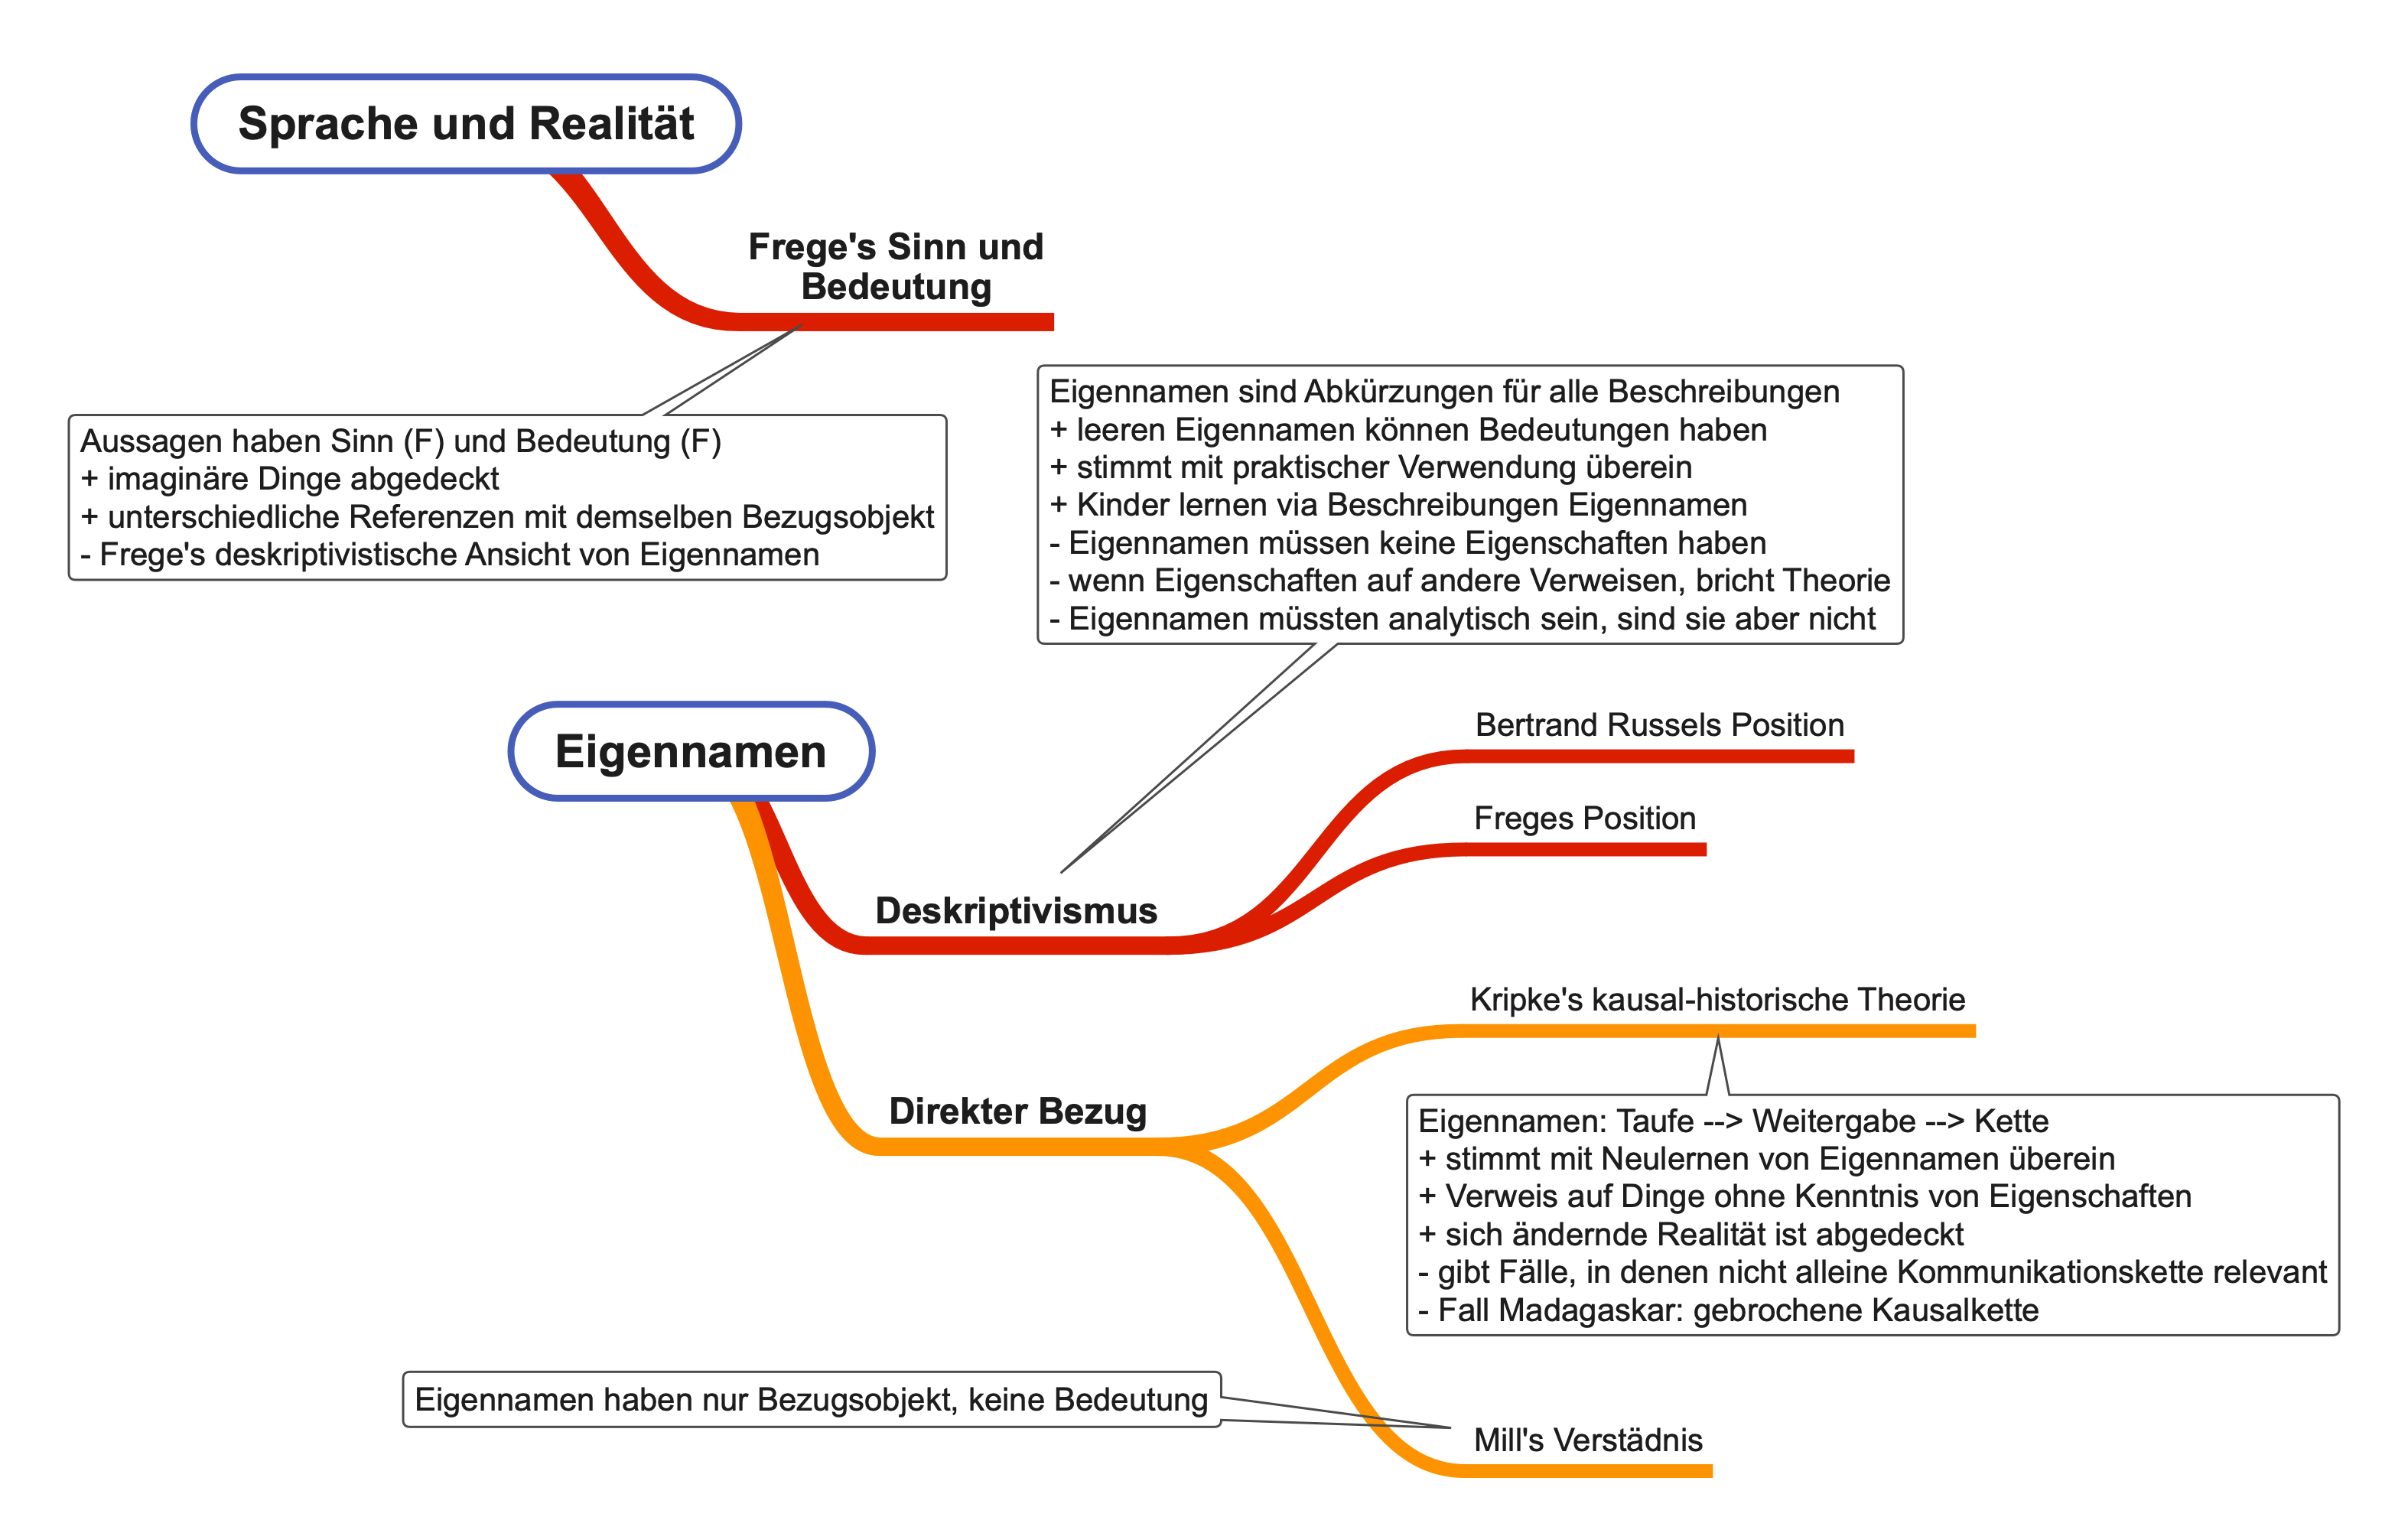
\includegraphics[width=\textwidth]{images/Sprache_und_Realitaet_Uebersicht.png}

\section{Bedeutung und Bezug}
In \ref{ChapterSpracheUndBedeutung} sind wir darauf gestossen, dass sprachliche Bedeutung und sprachlicher Bezug komplexer sein muss, als dies von der Gegenstandstheorie (\ref{SectionGegenstandstheorie}) oder der Gebrauchstheorie (\ref{SectionWittgensteinsGebrauchstheorie}) vorgeschlagen wird. Es stellt sich die Frage, wie es sich denn effektiv verhält. 

\section{Frege's Sinn und Bedeutung}\label{SectionFregesSinnUndBedeutung}
\begin{warningbox}
Frege erklärt die Bedeutung von Ausdrücken mit deren Sinn\textsubscript{F} ($\cong$ Eigenschaften/Merkmale/ausgedrückter Gedanke) und deren Bedeutung\textsubscript{F} ($\cong$ Bezugsgegenstand). 
\end{warningbox}


Gottlob Frege (1848-1925) gilt als Mitbegründer der modernen Logik und der analytischen Philosophie und hat die Welt der Philosophie erheblich beeinflusst. 

\paragraph{These} (1) Zwei Ausdrücke mit derselben Bedeutung\textsubscript{F} können unterschiedliche Sinne\textsubscript{F} haben, selbst wenn zwei Ausdrücke auf unterschiedliche Art denselben Gegenstand (Bedeutung\textsubscript{F}) meinen.
\paragraph{Erklärung} (Fast) jeder Ausdruck hat sowohl Bedeutung\textsubscript{F} ($\cong$ Bezugsgegenstand), wie auch Sinn\textsubscript{F} ($\cong$ Bedeutung). Dabei konstituiert der Fredsche Sinn\textsubscript{F} den Verweis (die Relation) und die Fredsche Bedeutung\textsubscript{F} das Objekt selber. In anderen Worten: Jeder Ausdruck besteht aus einem Bezug auf etwas und dem Objekt, worauf bezogen wird. 

Anhand des Bespieles <<Fido ist ein Hund>> lässt sich dies klarer aufzeigen; Die Bedeutung\textsubscript{F} ist der Bezugsgegenstand, also der Wahrheitswert der Aussage. Der Sinn\textsubscript{F} ist die Bedeutung der Aussage, also der ausgedrückte Gedanke, dass es eine wahre Relation zwischen Hund-Sein und dem Wesen gibt, welches als Fido (Eigennamen) bezeichnet wird.

\vspace{10pt} 
{\centering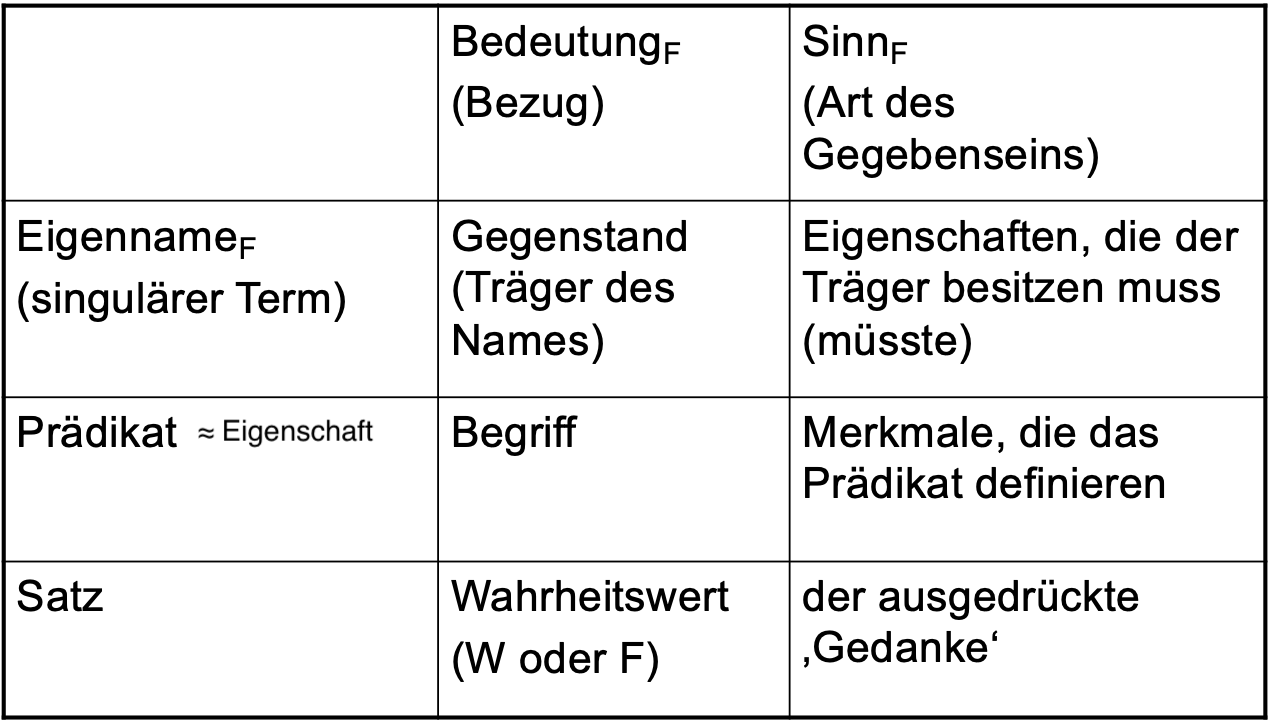
\includegraphics[height=5.5cm]{images/freges_sinn_und_bedeutung.png}\endcenter}

\paragraph{Argumente}
\begin{enumerate}
	\item Es ergeben sich zwei Vorteile gegenüber der einfachen Gegenstandstheorie (\ref{SectionGegenstandstheorie}): (1) Es lässt sich klären, wie Ausdrücke ohne Bedeutung\textsubscript{F} Sinn\textsubscript{F} besitzen können und (2) warum Identitätsaussagen oft informativ sind.
	\item Sätze/Aussagen mit \textbf{Sinn\textsubscript{F} ohne Bedeutung\textsubscript{F}} ($\cong$ Bedeutung ohne Bezug) werden durch Frege's Theorie abgedeckt. Dies ist zum Beispiel dann der Fall, wenn es um Ausdrücke wie <<die grösste natürliche Zahl>> handelt, die sich nicht auf einen (realen, tatsächlich existierenden) Gegenstand beziehen. Man nennt solche Ausdrücke \textit{leere singuläre Termini} oder \textit{leere Eigennahmen}. Trotz ihrem Bezug auf einen nichtrealen Gegenstand lässt sich der ausgedrückte Gedanke (Sinn\textsubscript{F}) hinter der Aussage/einem Satz, der eine solche \textit{leeren singulären Termini} (Sinn\textsubscript{F}) benutz, erfassen, ohne dass dieser einen Wahrheitswert (Bedeutung\textsubscript{F}) haben muss. 
	\item Auch die im Einwand \ref{EinwandDerMehrdeutigenBeschreibungGegenstandstheorie} der Gegenstandstheorie (\ref{SectionGegenstandstheorie}) angesprochenen verschiedenen Wege, wie auf ein und denselben Gegenstand verwiesen werden kann, wird durch Frege's Theorie gelöst. Beispielsweise verweisen <<der, mit den besten Zusammenfassungen>> oder <<der beste Student>> auf die gleichen Personen (Bedeutung\textsubscript{F}), diese werden aber durch andere Eigenschaften konstituiert (Sinn\textsubscript{F}). Aus den beiden Aussagen lässt sich lernen, dass ein und derselbe Bezugsgegenstand beide Eigenschaften erfüllt. 
\end{enumerate}

\paragraph{Einwände}
\begin{enumerate}
	\item Frege's Position gegenüber Eigennamen ist der Deskriptivismus. Also: Er ist davon überzeugt, dass, wenn man einen Eigennamen nennt, auch gleichzeitig alle Eigenschaften nennt, die auf den Bezugsgegenstand zutreffen. Im folgenden Teil der Zusammenfassung wird dies genauer erläutert. 
\end{enumerate}

\section{Eigennamen: Deskriptivismus}
Eigennamen sind Bestandteil der Menge aller \textit{singuläre Termini}. Doch wie ist ihr Bezug zur Realität und was bedeuten sie? Und hängen Bedeutung und Bezug von Eigennamen zusammen?

\paragraph{These} Eigennamen vereinen alle dem Bezugsobjekt zugeschrieben Eigenschaften in einer Art <<Abkürzung>>.

\subsection{Frege's Einstellung zu Eigennamen}
Wie sich aus Frege's Sinn und Bedeutung (\ref{SectionFregesSinnUndBedeutung}) ableiten lässt, vertritt er eine \textbf{deskriptivistische Position}; Eigennamen sind sowohl Bedeutung\textsubscript{F} ($\cong$ Bezugsgegenstand) wie auch Sinn\textsubscript{F} ($\cong$ Bedeutung). Dabei besteht der Sinn\textsubscript{F} aus allen Eigenschaften, die den Gegenstand besitzen muss, um Träger des Namens zu sein. Oder: Der Eigenname beschreibt seinen Träger als denjenigen mit Eigenschaften A, B, C, etc. So verweist z.B. der Name <<Andrin>> auf die Person, die alle Eigenschaften in sich vereint, die auf diese Person zutreffen. 

\subsection{Betrand Russell's deskriptivistische Position zu Eigennamen}
Ähnlich wie Gottlob Frege interpretiert auch Bertrand Russell (1872-1970) Eigennamen. Gemäss ihm sind gewöhnliche Eigennamen nichts anderes als \textit{Abkürzungen} für Kennzeichnungen (\textit{abbreviated definite descriptions}). So ist <<Nelson Mandela>> eine Abkürzung für <<der erste demokratisch gewählte Präsident Südafrikas>>. 

\paragraph{Argumente für den Deskriptivismus}
\begin{enumerate}
	\item Der Deskriptivismus kann leeren Eigennamen eine Bedeutung zuschreiben und somit aufzeigen, dass diese Eigennamen einen Informationsgehalt haben
	\item Fragt man nach einer Eigenschaft, die eindeutig einer Person zugeschrieben werden kann, so ist unsere Antwort jeweils den Eigennamen dieser Person. Dies ist ein Argument aus der Praxis. 
	\item Wenn Kinder die Eigennamen lernen, so lernen sie diese (im Allgemeinen) durch Beschreibungen/Kennzeichnungen, also über die Eigenschaften, die dem Bezugsobjekt des Eigennamen zugesprochen werden.
\end{enumerate}

\paragraph{Einwände gegen den Deskriptivismus}
\begin{enumerate}
	\item Kripke: Es gibt viele Fälle, bei denen Sprecher Eigennamen verwenden, ohne eine (spezifische) Kennzeichnung zu geben. Bsp. <<Guatemala ist \textit{ein} Land in Mittelamerika>>. Trotz dieser Uneindeutigkeit bezieht sich der Eigennamen auf ein bestimmtes Objekt. 
	\item Kripke: Erdenkt man sich ein Szenario, in welchem wir einen Eigennamen mit eindeutigen Eigenschaften verbinden, diese eindeutigen Eigenschaften aber in Wahrheit einem anderen Gegenstand zukommen lassen müsste, sprechen wir dann eigentlich von einer anderen Person? Bsp. Der Mathematiker Gödel hat das Unvollständigkeitsprinzip, für das er bekannt ist, von einer anderen Person gestohlen. Sprechen wir dann mit dem Satz <<Gödel hat das Unvollständigkeitsprinzip bewiesen>> eigentlich über die unbekannte Dritte Person?
	\item Wenn wir eine eindeutige Eigenschaft stark mit einem Eigennamen verbinden und dies in Form <<X ist Y>> ausdrücken (z.B. <<Washington ist die Hauptstadt der USA>>), dann müsste dieser Satz analytisch und somit notwendigerweise wahr sein. Dies ist aber nicht der Fall, denn, zumindest bei einigen eindeutigen Eigenschaften, der Wahrheitsgehalt kann sich ändern (z.B. wenn eine neue Hauptstadt bestimmt wird). Demzufolge kann der Eigennamen nicht eine Abkürzung für (eine Menge von) Eigenschaften sein. 
\end{enumerate}

\section{Eigennamen: Direkter Bezug (direkt referenzielle Theorien)}

\paragraph{These} Die Beziehung zwischen Eigennamen und dem Bezugsgegenstand ist nicht durch eine Kennzeichnung vermittelt, sondern \textit{direkt}.

\subsection{Jon Stuart Mill's Verständnis vom direkten Bezug}
Gemäss Jon Stuart Mill (1806-1873) haben Eigennamen eine \textit{Denotation} (= ein Bezugsobjekt), jedoch keine \textit{Konnotation} (= schreiben keine Eigenschaften zu).

\subsection{Saul Kripke's kausal-historische Theorie der Referenz}
Gemäss Saul Kripke (1940-2022, Pionier der Modallogik, Sprachphilosophie und Metaphysik) ist der Bezug (der Referent) eines Eigennamens historisch bzw. genealogisch bestimmt. D.h. (1) der Eigennamen wurde durch eine \textit{Taufe} eingeführt und (2) dieser wurde innerhalb einer Sprachgemeinschaft \textit{intentional} weitergegeben (\textit{kausal-historisch-intentionale Kommunikationskette}, die mit der \textit{Taufe} verbindet).

\paragraph{Argumente der kausal-historischen Theorie}
\begin{enumerate}
	\item Der Erwerb von Eigennamen wird von anderen, die den Namen verwenden, mit der Absicht kopiert, ihn gleich zu verwenden, wie die anderen.
	\item Die Theorie erlaubt den Bezug auf Dinge mittels deren Eigennamen, ohne viel darüber wissen zu müssen. 
	\item Die Theorie, weil sie nicht eine Eigenschaft stark mit einem Eigennamen verbindet, ist vereinbar mit einer sich ändernden Wirklichkeit. 
\end{enumerate}

\paragraph{Probleme der kausal-historischen Theorie}
\begin{enumerate}
	\item Kripke: Die Theorie scheint unzulänglich zu sein, denn es lassen sich Fälle kreieren, für die nicht \textit{allein} die Kommunikationskette relevant ist. Dies zum Beispiel im Falle von einem Bibliothekar, der seinen Hund Aristoteles genannt hat, wir bei der Verwendung diesen Namens aber ihn selber meinen. % TODO: bessers verständnis ufbaue für das biispil
	\item Kripke: Auch problematisch ist der Fall von <<Madagaskar>>. Entweder wir verwenden den Namen falsch und dieser bezieht sich eigentlich auf einen Küstenstreifen der afrikanischen Küste, oder, dies wäre gemäss der kausal-historischen Theorie, Marco Polo hat einen neuen Namen erschaffen für die Insel. Anders ausgedrückt: Die kausal-historische Theorie hat Mühe, wenn in der Überlieferungskette auf einmal ein Glied den Namen anders verwendet, als dies die Glieder vor ihm taten. 
\end{enumerate}

\end{document}